\documentclass[11pt,a4paper]{scrreprt}
\usepackage[applemac]{inputenc}
\usepackage{english}
\usepackage{graphicx}


%%% BEGIN DOCUMENT
\begin{document}
\begin{titlepage}

\begin{center}

\includegraphics[width=1\textwidth]{./bfh.png}\\[1cm]

\HRule \\[2cm]

{ \huge \bfseries Software Engineering and Design
		\\ \normalsize Solutions to the given tasks}
\\[0.4cm]
\HRule \\[5cm]



% Author and supervisor
\begin{minipage}{0.4\textwidth}
\begin{flushleft} \large
\emph{Authors:}\\
Maja \textsc{Kelterborn}, \\
Saskia \textsc{Basler}, \\
Rene \textsc{Vielgut}, \\
Rafael \textsc{Kapp}, \\
Adrian \textsc{Wyss}, \\
Patrick \textsc{Hirschi}
\end{flushleft}
\end{minipage}
\begin{minipage}{0.4\textwidth}
\begin{flushright} \large
\emph{Teacher:} \\
Dr. J�rgen \textsc{Vogel}
\end{flushright}
\end{minipage}

\vfill

% Bottom of the page
{\large \today}

\end{center}

\end{titlepage}
\tableofcontents

%%%%%%%%%%%%% Task 1 %%%%%%%%%%%%%%%%

\chapter{Task 01}
\section{Target Users}
\begin{itemize}
\item clinical staff
\item doctors
\item nurses
\item health visitors
\item receptionists
\item medical records staff
\end{itemize}

\section{Key Features}
\begin{itemize}
\item clinical staff: agenda, medical record
\begin{itemize}
\item doctors: descriptions, therapy records, instructions
\item nurses: therapy records, instructions
\item health visitors
\end{itemize}
\item receptionists: agenda
\item medical records staff: generating reports for management
\end{itemize}

\section{Critical Success Factors}
\textbf{Definition: }Terms for an element that are necessary for a project to achieve its mission.\footnote{en.wikipedia.org}
\begin{itemize}
\item focus on mental health care
\item data integrity
\item intuition
\end{itemize}

\section{Potential System Components and Architecture}
\begin{itemize}
\item database
\item interface usability 
\item user privileges management
\end{itemize}


%%%%%%%%%%%%% Task 2 %%%%%%%%%%%%%%%% 

\chapter{Task 02}
\section{Comparison \glqq plan-driven\grqq  vs. \glqq agile\grqq}
\subsection{Agile}
\textbf{positive points:}
\begin{itemize}
\item working and reacting on the needs of the users 
\item very flexible if changes are necessary to the project (simpler and easier)
\item is focused on the technical AND social problems of the project (customer involvement)
\item agile developing fits better for small teams
\item all members are involved in all parts (common knowledge)
\end{itemize}
\textbf{negative point:}
\begin{itemize}
\item no clear contact person on the developer side
\end{itemize}
\subsection{Plan-driven}
\textbf{positive point:}
\begin{itemize}
\item clear structure of the software allows easy task assigning (team)
\end{itemize}
\textbf{negative points:}
\begin{itemize}
\item very unflexible system if changes are necessary (customer)
\item finding functions, which are also needed, after testing first release, will be expensive to implement (the client probably is not equal the user) (customer)
\item very certain, that a new software is needed, at the moment, the old system gets delivered (to much other & new functions needed) (customer)
\end{itemize}
\subsection{Conclusion}
Because of the previously seen slides, we came to the conclusion that we are going to use an agile development system. According to our knowledge at the moment we will use XtremeProgramming. For questions on the part of the customer, we nominated Mr. Rafael Kapp as the central contact person.
\section{Process Model}
\scalebox{0.4}{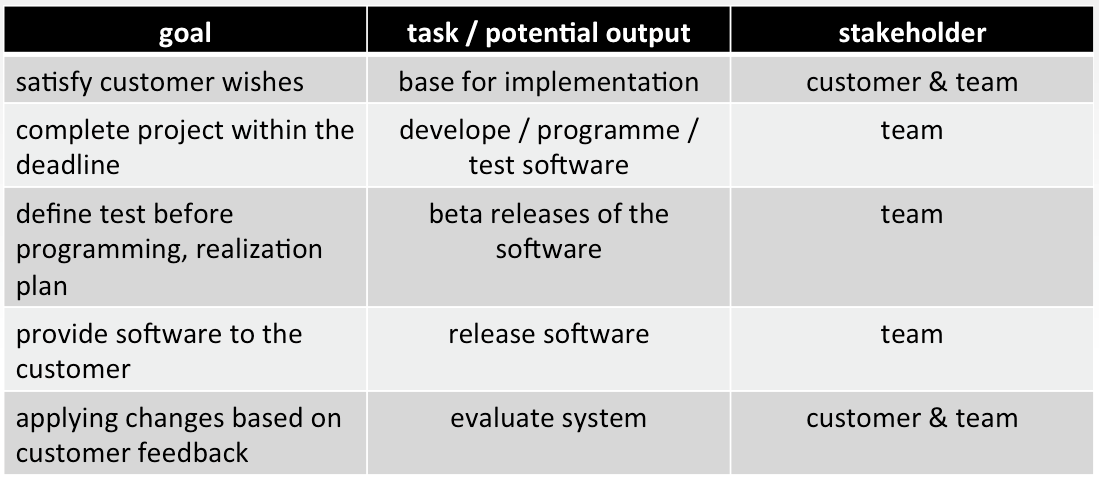
\includegraphics{./processmodel.png}}

%%%%%%%%%%%%%%%%%%%%%%%%%%%%%%%

\end{document}

